\documentclass{amsart}

\usepackage[T1]{fontenc}
\usepackage{enumerate, amsmath, amsfonts, amssymb, amsthm, mathrsfs, wasysym, graphics, graphicx, xcolor, url, hyperref, hypcap, xargs, multicol, overpic, pdflscape, multirow, hvfloat, array, ae, aecompl, pifont, mathtools, a4wide}
\usepackage{marginnote}
\hypersetup{colorlinks=true, citecolor=darkblue, linkcolor=darkblue}
\usepackage[all]{xy}
%\usepackage[bottom]{footmisc}
\usepackage{tikz}
\usepackage{tkz-graph}
\usetikzlibrary{trees, decorations, decorations.markings, shapes, arrows, matrix, calc, fit, intersections, patterns, angles}
\graphicspath{{figures/}}
\makeatletter\def\input@path{{figures/}}\makeatother
\usepackage{caption}
\captionsetup{width=\textwidth}

%%%%%%%%%%%%%%%%%%%%%%%%%%%%%%%%%%%%%%

% theorems
\newtheorem{theorem}{Theorem}[]
\newtheorem{corollary}[theorem]{Corollary}
\newtheorem{proposition}[theorem]{Proposition}
\newtheorem{lemma}[theorem]{Lemma}
\newtheorem{conjecture}[theorem]{Conjecture}
\newtheorem*{theorem*}{Theorem}%[section]

\theoremstyle{definition}
\newtheorem{definition}[theorem]{Definition}
\newtheorem{example}[theorem]{Example}
\newtheorem{remark}[theorem]{Remark}
\newtheorem{question}[theorem]{Question}
\newtheorem{notation}[theorem]{Notation}
\newtheorem{assumption}[theorem]{Assumption}
\newtheorem{convention}[theorem]{Convention}

% math special letters
\newcommand{\R}{\mathbb{R}} % reals
\newcommand{\N}{\mathbb{N}} % naturals
\newcommand{\Z}{\mathbb{Z}} % integers
\newcommand{\C}{\mathbb{C}} % complex
\newcommand{\I}{\mathbb{I}} % set of integers
\newcommand{\HH}{\mathbb{H}} % hyperplane
\newcommand{\K}{k} % field
\newcommand{\fA}{\mathfrak{A}} % alternating group
\newcommand{\fS}{\mathfrak{S}} % symmetric group
\newcommand{\cA}{\mathcal{A}} % algebra
\newcommand{\cC}{\mathcal{C}} % collection
\newcommand{\cS}{\mathcal{S}} % ground set
\newcommand{\uR}{\underline{R}} % underline set
\newcommand{\uS}{\underline{S}} % underline set
\newcommand{\uT}{\underline{T}} % underline set
\newcommand{\oS}{\overline{S}} % overline set
\newcommand{\ucS}{\underline{\cS}} % underline ground set
\renewcommand{\b}[1]{\mathbf{#1}} % bold letters
\newcommand{\h}{\widehat} % hat letters

% math commands
\newcommand{\set}[2]{\left\{ #1 \;\middle|\; #2 \right\}} % set notation
\newcommand{\bigset}[2]{\big\{ #1 \;\big|\; #2 \big\}} % big set notation
\newcommand{\Bigset}[2]{\Big\{ #1 \;\Big|\; #2 \Big\}} % Big set notation
\newcommand{\setangle}[2]{\left\langle #1 \;\middle|\; #2 \right\rangle} % set notation
\newcommand{\ssm}{\smallsetminus} % small set minus
\newcommand{\dotprod}[2]{\left\langle \, #1 \; \middle| \; #2 \, \right\rangle} % dot product
\newcommand{\symdif}{\,\triangle\,} % symmetric difference
\newcommand{\one}{{1\!\!1}} % the all one vector
\newcommand{\eqdef}{\mbox{\,\raisebox{0.2ex}{\scriptsize\ensuremath{\mathrm:}}\ensuremath{=}\,}} % :=
\newcommand{\defeq}{\mbox{~\ensuremath{=}\raisebox{0.2ex}{\scriptsize\ensuremath{\mathrm:}} }} % =:
\newcommand{\simplex}{\triangle} % simplex
\renewcommand{\implies}{\Rightarrow} % imply sign
\newcommand{\transpose}[1]{{#1}^t} % transpose matrix

% operators
\DeclareMathOperator{\conv}{conv} % convex hull
\DeclareMathOperator{\vect}{vect} % linear span
\DeclareMathOperator{\cone}{cone} % cone hull
\DeclareMathOperator{\inv}{inv} % inversions
\DeclareMathOperator{\ascents}{asc} % ascents
\DeclareMathOperator{\descents}{des} % descents

% others
\newcommand{\fref}[1]{Figure~\ref{#1}} % reference figures
\newcommand{\ie}{\textit{i.e.}~} % id est
\newcommand{\eg}{\textit{e.g.}~} % exempli gratia
\newcommand{\Eg}{\textit{E.g.}~} % exempli gratia
\newcommand{\apriori}{\textit{a priori}} % a priori
\newcommand{\viceversa}{\textit{vice versa}} % vice versa
\newcommand{\versus}{\textit{vs.}~} % versus
\newcommand{\aka}{\textit{a.k.a.}~} % also known as
\newcommand{\perse}{\textit{per se}} % per se
\newcommand{\ordinal}{\textsuperscript{th}} % th for ordinals
\newcommand{\ordinalst}{\textsuperscript{st}} % st for ordinals
\definecolor{darkblue}{rgb}{0,0,0.7} % darkblue color
\definecolor{green}{RGB}{57,181,74} % green color
\definecolor{violet}{RGB}{147,39,143} % violet color
\newcommand{\darkblue}{\color{darkblue}} % darkblue command
\newcommand{\defn}[1]{\textsl{\darkblue #1}} % emphasis of a definition
\newcommand{\para}[1]{\medskip\noindent\textbf{#1.}} % paragraph
\renewcommand{\topfraction}{1} % possibility to have one page of pictures
\renewcommand{\bottomfraction}{1} % possibility to have one page of pictures
%\renewcommand\labelitemi{$\diamond$} % redefine itemize default symbol
\newcommand{\ex}{_{\textrm{exm}}} % examples
\newcommand{\pa}{_{\textrm{pa}}} % path

% marginal comments
\usepackage{todonotes}
\newcommand{\yann}[1]{\textbf{#1 --- Y.}} % {\todo[color=red!30]{#1 \\ \hfill --- Y.}}
\newcommand{\vincent}[1]{\todo[color=blue!30]{#1 \\ \hfill --- V.}}
\newcommand{\pierreguy}[1]{\todo[color=green!30]{#1 \\ \hfill --- PG.}}

% SPECIFIC NON-KISSING COMPLEX

% COMBINATORICS
% quiver
\newcommand{\blossom}{^\text{\ding{96}}} % blossom
\newcommand{\blinkers}[1]{_{\LEFTCIRCLE \!\! #1 \!\! \RIGHTCIRCLE}} % blossom
\newcommand{\indeg}{\mathrm{indeg}} % in-degree
\newcommand{\outdeg}{\mathrm{outdeg}} % out-degree
%\newcommand{\tai}{\mathsf{tai}} % target incompatible
%\newcommand{\tac}{\mathsf{tac}} % target compatible
%\newcommand{\soi}{\mathsf{soi}} % source incompatible
%\newcommand{\soc}{\mathsf{soc}} % source compatible
%\newcommand{\cso}{\mathsf{cso}} % cosource
%\newcommand{\cta}{\mathsf{cta}} % cotarget

% walks
\newcommand{\strings}{\mathcal{S}} % strings
\newcommand{\distinguishableStrings}{\mathcal{S}_\mathrm{dist}} % distinguishable strings
\newcommand{\lfStrings}{\underline{\mathcal{S}}} % loop-free strings
\newcommand{\walks}{\mathcal{W}} % walks
\newcommand{\straightWalks}{\mathcal{W}_\mathrm{str}} % straight walks
\newcommand{\bendingWalks}{\mathcal{W}_\mathrm{bend}} % bending walks
\newcommand{\NKWalks}{\mathcal{W}_\mathrm{nk}} % non-kissing walks
\newcommand{\peaks}[1]{\mathsf{peaks}(#1)} % peaks
\newcommand{\deeps}[1]{\mathsf{deeps}(#1)} % deeps
\newcommand{\distinguishedWalk}[2]{\mathsf{dw}(#1,#2)} % distinguished walk
\newcommand{\distinguishedArrows}[2]{\mathsf{da}(#1,#2)} % distinguished arrows
\newcommand{\distinguishedString}[2]{\mathsf{ds}(#1,#2)} % distinguished string
\newcommand{\distinguishedSign}[2]{\varepsilon(#1,#2)} % distinguished sign

% non-kissing complex, lattice, flip graph
\newcommand{\kn}{\kappa} % kissing number
\newcommand{\KN}{\textsc{kn}} % Kissing Number
\newcommandx{\NKC}[1][1=\bar Q]{\mathcal{K}_{\mathrm{nk}}(#1)} % non-kissing complex
\newcommandx{\RNKC}[1][1=\bar Q]{\mathcal{C}_{\mathrm{nk}}(#1)} % non-kissing complex
\newcommandx{\NKL}[1][1=\bar Q]{\mathcal{L}_{\mathrm{nk}}(#1)} % non-kissing lattice
\newcommandx{\NKG}[1][1=\bar Q]{\mathcal{G}_{\mathrm{nk}}(#1)} % non-kissing flip graph
\newcommandx{\NFC}[1][1=\bar Q]{\mathcal{C}_{\mathrm{nf}}(#1)} % non-friendly complex
\newcommand{\peak}{\mathrm{peak}} % bottom dissection
\newcommand{\deep}{\mathrm{deep}} % top dissection
\newcommand{\reversed}[1]{#1^{\mathrm{rev}}} % reverse all arrows
\renewcommand{\top}{\mathrm{top}} % top
\newcommand{\bottom}{\mathrm{bot}} % bottom

% accordion and slalom complexes
\newcommand{\surface}{\mathcal{S}} % an orientable surface
\newcommand{\dual}{^*} % duality
\newcommand{\dissection}{\mathrm{D}} % dissection of a marked surface
\newcommand{\vertices}{\mathcal{V}} % vertices of a dissection
\newcommand{\edges}{\mathcal{E}} % edges of a dissection
\newcommand{\faces}{\mathcal{F}} % faces of a dissection
\renewcommandx{\AC}[1][1=\dissection]{\mathcal{K}_{\mathrm{acc}}(#1)} % accordion complex
\newcommandx{\RAC}[1][1=\dissection]{\mathcal{C}_{\mathrm{acc}}(#1)} % reduced accordion complex
\newcommandx{\SC}[1][1=\dissection\dual]{\mathcal{K}_{\mathrm{sla}}(#1)} % slalom complex
\newcommandx{\RSC}[1][1=\dissection\dual]{\mathcal{C}_{\mathrm{sla}}(#1)} % reduced slalom complex
\newcommandx{\NCC}[1][1={\dissection, \dissection\dual}]{\mathcal{K}_{\mathrm{nc}}(#1)} % non-crossing complex
\newcommandx{\RNCC}[1][1={\dissection, \dissection\dual}]{\mathcal{C}_{\mathrm{nc}}(#1)} % non-crossing complex

% lattices
\newcommand{\meet}{\wedge} % meet
\newcommand{\join}{\vee} % join
\newcommand{\bigMeet}{\bigwedge} % meet
\newcommand{\bigJoin}{\bigvee} % join
\newcommand{\closure}[1]{#1^{\mathrm{cl}}} % closure operator
\newcommand{\coclosure}[1]{#1^{\mathrm{cocl}}} % coclosure operator
\newcommand{\uclosure}[1]{#1^{\underline{\mathrm{cl}}}} % loop free closure operator
\newcommand{\Bicl}[1]{\mathsf{Bic}(#1)} % biclosed sets
\newcommand{\projDown}{\pi_\downarrow} % down projection map
\newcommand{\projUp}{\pi^\uparrow} % up projection map
\newcommand{\JI}{\mathsf{JI}} % join-irreducible
\newcommand{\MI}{\mathsf{MI}} % meet-irreducible
\newcommand{\Cong}{\mathsf{Cong}} % congruence lattice
\newcommand{\con}{\mathrm{con}} % congruence contracting a cover relation
\newcommand{\ji}{\mathsf{ji}} % join irreducible
\newcommand{\mi}{\mathsf{mi}} % meet irreducible

% GEOMETRY
% g-vectors
\newcommand{\gvector}[1]{\mathbf{g}(#1)} % g-vector of the path #1
\newcommand{\gvectors}[1]{\mathbf{g}(#1)} % g-vectors of the paths #1
\newcommandx{\gvectorFan}[1][1=\bar Q]{\mathcal{F}^\mathbf{g}(#1)} % g-vector fan
% c-vectors
\newcommand{\cvector}[2]{\mathbf{c}(#1 \in #2)} % c-vector of the path #1 in the facet #2
\newcommand{\cvectors}[1]{\mathbf{c}(#1)} % c-vectors of the paths #1
\newcommandx{\allcvectors}[1][1=\bar Q]{\mathbf{C}(#1)} % all c-vectors with respect to the initial cluster #1
\newcommandx{\cvectorFan}[1][1=\bar Q]{\mathcal{F}^\mathbf{c}(#1)} % fan of hyperplanes orthogonal to all c-vectors
% points, hyperplanes, half-spaces
\newcommand{\point}[1]{\mathbf{p}(#1)} % vertex of the grid associahedron corresponding to the cluster #1
\newcommand{\ray}{\mathbf{r}} % ray
\newcommand{\rays}{\mathbf{R}} % rays
\newcommand{\hs}{\mathbf{H}^{\le}} % half space
\newcommand{\HS}[1]{\mathbf{H}^{\le}(#1)} % half space
\newcommand{\hyp}{\mathbf{H}^{=}} % hyperplane
\newcommand{\Hyp}[1]{\mathbf{H}^{=}(#1)} % hyperplane
\newcommand{\fix}[1]{\mathrm{Fix}(#1)} % fix space
% polytopes
\newcommandx{\Asso}[2][1=\bar Q,2={}]{\mathsf{Asso}^{#2}(#1)} % associahedron
\newcommandx{\Zono}[2][1=\bar Q,2={}]{\mathsf{Zono}^{#2}(#1)} % zonotope
\newcommand{\Fan}{\mathcal{F}} % fan
\newcommand{\multiplicityVector}{\b{m}} % multiplicity vector

% ALGEBRA
\newcommand{\Hom}[1]{\operatorname{{\rm Hom}}_{#1}}
\newcommand{\Ext}[1]{\operatorname{{\rm Ext}}_{#1}}
\newcommandx{\AR}[1][1=\bar Q]{\mathrm{AR}(#1)} % Auslander-Reiten quiver
\newcommandx{\tTC}[1][1=\bar Q]{\mathcal{K}^{\textrm{s$\tau$-tilt}}(#1)} % tau-tilting complex
\newcommand{\rep}{\operatorname{{\rm rep}}}
\newcommand{\proj}{\operatorname{{\rm proj}}}

%% formating the part command
%\makeatletter
%\def\part{\@startsection{part}{1}%
%\z@{.7\linespacing\@plus\linespacing}{.8\linespacing}%
%{\LARGE\sffamily\centering}}
%\@addtoreset{section}{part}
%\makeatother
%\renewcommand{\thesection}{\arabic{part}.\arabic{section}}

% formating the table of contents
\makeatletter
\def\l@section{\@tocline{1}{2pt}{0pc}{}{}}
\makeatother
\let\oldtocpart=\tocpart
\renewcommand{\tocpart}[2]{\bf\large\oldtocpart{#1}{#2}}
\let\oldtocsection=\tocsection
\renewcommand{\tocsection}[2]{\bf\oldtocsection{#1}{#2}}

%%%%%%%%%%%%%%%%%%%%%%%%%%%%%%%%%%%%%%

\title[Non-kissing and non-crossing complexes for gentle algebras]{Non-kissing and non-crossing complexes \\ for gentle algebras}

\thanks{YP, VP and PGP were partially supported by the French ANR grant SC3A~(15\,CE40\,0004\,01).}

\author{Yann Palu}
\address[Yann Palu]{LAMFA, Universit\'e Picardie Jules Verne, Amiens}
\email{yann.palu@u-picardie.fr}
\urladdr{\url{http://www.lamfa.u-picardie.fr/palu/}}

\author{Vincent Pilaud}
\address[Vincent Pilaud]{CNRS \& LIX, \'Ecole Polytechnique, Palaiseau}
\email{vincent.pilaud@lix.polytechnique.fr}
\urladdr{\url{http://www.lix.polytechnique.fr/~pilaud/}}

\author{Pierre-Guy Plamondon}
\address[Pierre-Guy Plamondon]{Laboratoire de Math\'ematiques d'Orsay, Universit\'e Paris-Sud, CNRS, Universit\'e Paris-Saclay}
\email{pierre-guy.plamondon@math.u-psud.fr}
\urladdr{\url{https://www.math.u-psud.fr/~plamondon/}}

\author{Sibylle Schroll}
\address[Sibylle Schroll]{}
\email{schroll@leicester.ac.uk}
\urladdr{\url{}}

%%%%%%%%%%%%%%%%%%%%%%%%%%%%%%%%%%%%%%

\begin{document}

\begin{abstract}
We consider three combinatorial models for the support $\tau$-tilting complex of a gentle bound quiver: the accordion complex, the slalom complex, and the non-kissing complex. We unify these models in the same picture.
\end{abstract}

%\vspace*{.3cm}

\maketitle

Possible titles, depending on what we want to insist on:
\begin{enumerate}
\item Accordion / slalom / non-kissing / support $\tau$-tilting complexes all coincide for gentle algebras
\item Non-kissing and non-crossing complexes for gentle algebras
\item Combinatorial models for support $\tau$-tilting on gentle algebras: accordion, slalom and non-kissing complexes
\end{enumerate}


\section{Non-kissing complex}

\subsection{Gentle bound quivers and their blossoming quivers}

We consider a \defn{bound quiver}~$\bar Q = (Q,I)$, formed by a quiver~$Q$ and an admissible ideal~$I$ of the path algebra~$kQ$, so that the quotient algebra~$kQ/I$ is finite dimensional.

\begin{definition}[\cite{ButlerRingel}]
\label{def:gentleQuiver}
A \defn{gentle bound quiver}~$\bar Q \eqdef (Q,I)$ is a bound quiver such that
\begin{itemize}
\item each vertex~$v \in Q_0$ has at most two incoming and two outgoing arrows,
\item the ideal~$I$ is generated by paths of length exactly two,
\item for any arrow~$\beta \in Q_1$, there is at most one arrow~$\alpha \in Q_1$ such that~$t(\alpha) = s(\beta)$ and~${\alpha\beta\notin I}$ (resp.~$\alpha\beta \in I$) and at most one arrow~$\gamma \in Q_1$ such that~$t(\beta) = s(\gamma)$~and~${\beta\gamma\notin I}$~(resp.~${\beta\gamma \in I}$).
\end{itemize}
The algebra~$kQ/I$ is called a \defn{gentle algebra}.
\end{definition}

\begin{definition}[\cite{PaluPilaudPlamondon}]
\label{def:blossomingQuiver}
A gentle bound quiver~$\bar Q$ is \defn{complete} if any vertex~$v \in Q_0$ is incident to either one ($v$ is a leaf) or four arrows ($v$ is an internal vertex).
The \defn{pruned subquiver} of a quiver $\bar Q$ is the gentle quiver obtained by deleting all leaves of~$\bar Q$ (degree one vertices) and their incident arrows.
The \defn{blossoming quiver} of a gentle bound quiver~$\bar Q$ is the complete gentle bound quiver~$\bar Q\blossom$ whose pruned subquiver is~$\bar Q$.
The vertices of~$Q\blossom_0 \ssm Q_0$ are called \defn{blossom vertices}, and the arrows~$Q\blossom_1 \ssm Q_1$ are called \defn{blossom arrows}.
\end{definition}

\vincent{Examples}
\vincent{Should we introduce Koszul duality here and say what it does on quivers?}

\subsection{Strings and walks}

\begin{definition}
\label{def:string}
Let~$\bar Q = (Q,I)$ be a gentle bound quiver.
A \defn{string} for~$\bar Q$ is a word of the form
\(
\rho = \alpha_1^{\varepsilon_1}\alpha_2^{\varepsilon_2}\cdots \alpha_\ell^{\varepsilon_\ell},
\)
where
	\begin{itemize}
	\item $\alpha_i \in Q_1$ and~$\varepsilon_i \in \{-1,1\}$ for all~$i \in [\ell]$,
	\item $t(\alpha_i^{\varepsilon_i}) = s(\alpha_{i+1}^{\varepsilon_{i+1}})$ for all~$i \in [\ell-1]$,
	\item there is no path~$\pi \in I$ such that~$\pi$ or~$\pi^{-1}$ appears as a factor of~$\rho$, and
	\item $\rho$ is reduced, in the sense that no factor~$\alpha\alpha^{-1}$ or~$\alpha^{-1}\alpha$ appears in~$\rho$, for~$\alpha \in Q_1$.
	\end{itemize}
The integer~$\ell$ is called the \defn{length} of the string~$\rho$.
We let~$s(\rho) \eqdef s(\alpha_1^{\varepsilon_1})$ and~$t(\rho) \eqdef t(\alpha_\ell^{\varepsilon_\ell})$ denote the source and target of~$\rho$.
For each vertex~$v \in Q_0$, there is also a \defn{string of length zero}, denoted by~$\varepsilon_v$, that starts and ends at~$v$.
%We denote by~$\strings(\bar Q)$ the set of strings on~$\bar Q$.
%We usually denote strings by~$\rho, \sigma, \tau$.
We often implicitly identify the two inverse strings~$\rho$ and~$\rho^{-1}$, and we let~$\strings^\pm(\bar Q) \eqdef \set{\{\rho, \rho^{-1}\}}{\rho \in \strings(\bar Q)}$ denote the collection of all \defn{undirected strings} of~$\bar Q$.

%We call \defn{negative simple string} a formal word of length zero of the form $-v$, where $v$ is any vertex of $Q_0$. We denote by
%\(
%\strings^\pm_{\ge -1}(\bar Q) \eqdef \strings^\pm(\bar Q) \sqcup \set{-v}{v \in Q_0}
%\)
%the set of \defn{almost positive unoriented strings}.
%Note that~$\varepsilon_v$ and~$-v$ are different almost positive strings.
%\end{enumerate}
\end{definition}

\begin{definition}
\label{def:walk}
A \defn{walk} of a gentle quiver~$\bar Q$ is a maximal string of its blossoming quiver~$\bar Q \blossom$ (thus joining two blossom vertices of~$\bar Q \blossom$).
We denote by~$\walks(\bar Q)$ the set of all walks on~$\bar Q$.
As for strings, we implicitly identify the two inverse walks~$\omega$ and~$\omega^{-1}$, and we let~$\walks^\pm(\bar Q) \eqdef \set{\{\omega, \omega^{-1}\}}{\omega \in \walks(\bar Q)}$ denote the set of \defn{undirected walks} of~$\bar Q$.
\end{definition}

\begin{definition}
\label{def:substrings}
A \defn{substring} of a walk~$\omega = \alpha_1^{\varepsilon_1} \dots \alpha_\ell^{\varepsilon_\ell} \in \walks(\bar Q)$ is a string~$\sigma = \alpha_i^{\varepsilon_i} \dots \alpha_j^{\varepsilon_j}$ of~$\strings(\bar Q)$ for some~$1 < i \le j < \ell$.
Note that 
\begin{itemize}
\item the endpoints of~$\sigma$ are not allowed to be the blossom endpoints of~$\omega$,
\item the position of~$\sigma$ as a factor of~$\omega$ matters (the same string at a different position is considered a different substring),
\item the string~$\varepsilon_v$ is a substring of~$\omega$ for each occurence of~$v$ as a vertex of~$\omega$.
\end{itemize}
The substring~$\sigma = \alpha_i^{\varepsilon_i} \dots \alpha_j^{\varepsilon_j}$ is \defn{at the bottom} (resp.~\defn{on top}) of the walk~$\omega = \alpha_1^{\varepsilon_1} \dots \alpha_\ell^{\varepsilon_\ell}$ if~$\varepsilon_{i-1} = 1$ and~$\varepsilon_{j+1} = -1$ (resp.~if~$\varepsilon_{i-1} = -1$ and~$\varepsilon_{j+1} = 1$), that is, the two arrows of~$\omega$ incident to the endpoints of~$\sigma$ point towards~$\sigma$ (resp.~outwards from~$\sigma$).
We let~$\Sigma(\omega)$ be the set of substrings of~$\omega$ and~$\Sigma_\bottom(\omega)$ and~$\Sigma_\top(\omega)$ be the sets of bottom and top substrings of~$\omega$ respectively.
We use the same notations for undirected walks (of course, substrings of an undirected walk are undirected).
\end{definition}

\begin{definition}
\label{def:straightBended}
A \defn{peak} (resp.~\defn{deep}) of a walk~$\omega$ is a substring of~$\omega$ of length zero which is on top (resp.~at the bottom of~$\omega$).
A \defn{corner} is either a peak or a deep (in other words, it is a vertex of~$\omega$ where the arrows change direction).
A walk~$\omega$ is \defn{straight} if it has no corner (\ie if~$\omega$ or~$\omega^{-1}$ is a path in~$\bar Q\blossom$), and \defn{bending} otherwise. Let $\straightWalks(\bar Q)$ and~$\bendingWalks(\bar Q)$ denote the sets of straight and bending walks of~$\bar Q$ and let~$\straightWalks^\pm(\bar Q) \eqdef \set{\{\omega, \omega^{-1}\}}{\omega \in \straightWalks(\bar Q)}$ and~$\bendingWalks^\pm(\bar Q) \eqdef \set{\{\omega, \omega^{-1}\}}{\omega \in \bendingWalks(\bar Q)}$.
A \defn{peak walk} (resp.~\defn{deep walk}) is a walk with a unique corner (in other words, it switches orientation only once), which is a peak (resp.~deep). For~$v \in Q_0$, we denote by~$v_\peak$ the peak walk with peak at~$v$ and by~$v_\deep$ the deep walk with deep~at~$v$.
\end{definition}

\subsection{Non-kissing complex}

\begin{definition}
\label{def:kiss}
Let~$\omega,\omega' \in \walks^\pm(\bar Q)$ be two undirected walks on~$\bar Q$.
We say that~$\omega$ \defn{kisses}~$\omega'$ if~$\Sigma_\top(\omega) \cap \Sigma_\bottom(\omega') \ne \varnothing$.
See \fref{fig:kissingCrossing}.
% \ie if there exist a common substring~$\sigma \in \strings^\pm(\bar Q)$ of~$\omega$ and~$\omega'$ such that the arrows of~$\omega$ incident to~$\sigma$ are both outgoing while the arrows of~$\omega'$ incident to~$\sigma$ are both incoming.
We say that~$\omega$ and~$\omega'$ are \defn{kissing} if~$\omega$ kisses~$\omega'$ or~$\omega'$ kisses~$\omega$ (or both).
Note that we authorize the situation where~$\sigma$ is reduced to a vertex~$v$, meaning that~$v$ is a peak of~$\omega$ and a deep of~$\omega'$.
Observe also that~$\omega$ can kiss~$\omega'$ several times, that~$\omega$ and~$\omega'$ can mutually kiss, and that~$\omega$ can kiss itself.
We denote by~$\NKWalks(\bar Q)$ the walks on~$\bar Q$ which are not self-kissing and by~$\NKWalks^\pm(\bar Q) \eqdef \set{\{\omega, \omega^{-1}\}}{\omega \in \NKWalks(\bar Q)}$ their undirected version.
\end{definition}

\begin{figure}
	\capstart
	\centerline{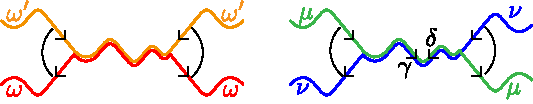
\includegraphics[scale=1]{kissingCrossing}}
	\caption{A schematic representation of two kissing walks (left) and two crossing walks~(right): $\omega$~kisses~$\omega'$ (left) while~$\mu$~crosses~$\nu$ (right). For the crossing walks, we have~$\mu \prec_\gamma \nu$ while~$\nu \prec_\delta \mu$.}
	\label{fig:kissingCrossing}
\end{figure}

\begin{definition}
\label{def:nKc}
The \defn{non-kissing complex} of~$\bar Q$ is the simplicial complex~$\NKC$ whose faces are the collections of pairwise non-kissing walks of~$\NKWalks^\pm(\bar Q)$.
Note that self-kissing walks never appear in~$\NKC$ by definition.
In contrast, no straight walk can kiss another walk by definition, so that they appear in all facets of~$\NKC$.
We thus consider the \defn{reduced non-kissing complex}~$\RNKC$ to be the deletion of all straight walks from~$\NKC$.
\end{definition}

\begin{theorem}[{\cite[Cor.~2.27 \& Cor.~2.33]{PaluPilaudPlamondon}}]
The reduced non-kissing complex~$\RNKC$ is pure of dimension~$|Q_0|$ (\ie all maximal faces have dimension~$|Q_0|$) and thin (\ie all codimension~$1$ faces are contained in exactly two facets).
\end{theorem}

This result follows from the existence of flips in non-kissing facets.
This operation is illustrated in \fref{fig:flip}.

\begin{figure}[t]
	\capstart
	\centerline{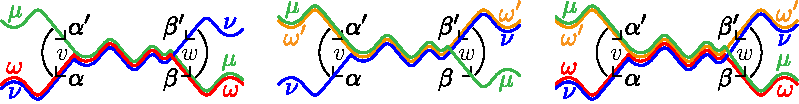
\includegraphics[scale=1]{flip}}
	\caption{A schematic representation of flips in the non-kissing complex. The flip exchanges the walk~$\omega = \rho \sigma \tau$ in the facet~$F$ (left) with the walk~$\omega' = \rho' \sigma \tau'$ in the facet~$F'$ (middle), using the walks~$\mu = \rho' \sigma \tau$ and~$\nu = \rho \sigma \tau'$. The walk~$\omega'$ kisses~$\omega$ but no other walk of~$F$ (right).}
	\label{fig:flip}
\end{figure}

\section{Accordion complex, slalom complex, and non-crossing complex}

\subsection{Dual dissections of a surface}

\begin{definition}
A \defn{marked surface}~$\bar\surface \eqdef (\surface, M)$ is an orientable surface~$\surface$ with boundaries, together with a set~$M$ of marked points which can be on the boundary of~$\surface$ or not.
For~$V \subset \surface$, a \defn{$V$-arc} on~$\bar\surface$ is a curve on~$\surface$ connecting two points of~$V$ and whose interior is disjoint from~$M$ and the boundary of~$\surface$.
As usual, arcs are considered up to homotopy relative to their endpoints in~$\surface \ssm M$, and curves homotopic to a boundary are not allowed.
Two arcs \defn{cross} when they intersect in~their~interior.
\end{definition}

\begin{definition}
A \defn{dissection} of~$\bar\surface$ is a collection~$\dissection$ of pairwise non-crossing arcs on~$\bar\surface$.
The \defn{edges} of~$\dissection$ are its arcs together with the boundary arcs of~$\bar\surface$.
The \defn{faces} of~$\dissection$ are the connected components of the complement of the union of the edges of~$\dissection$ in the surface~$\surface$.
We denote by~$\vertices(\dissection)$, $\edges(\dissection)$ and~$\faces(\dissection)$ the sets of vertices, edges and faces of~$\dissection$ respectively.
The dissection~$\dissection$ is \defn{cellular} if all its faces are disks.
For~$V \subseteq M$, a \defn{$V$-dissection} is a dissection with only $V$-arcs.
\end{definition}

\begin{convention}
\textbf{All throughout the paper, all dissections are considered cellular.}
The case of non-cellular dissections will be discussed in Section~\ref{sec:nonCellularDissections}.
\end{convention}

\begin{definition}
Consider a marked surface~$\bar\surface = (\surface, V \sqcup V\dual)$, where~$V$ and~$V\dual$ are two disjoint sets of marked points so that the points of~$V$ and~$V\dual$ that are on the boundary of~$\surface$ alternate.
A cellular $V$-dissection~$\dissection$ of~$\bar\surface$ and a cellular $V\dual$-dissection~$\dissection\dual$ of~$\bar\surface$ are \defn{dual cellular dissections} if there are pairs of mutually inverse bijections~$V\dual \leftrightarrow \faces(\dissection)$ and~$V \leftrightarrow \faces(\dissection\dual)$, denoted~$\dual$ in both directions, such that~$\dissection$ has an edge joining its vertices~$u,v \in V$ and separating its faces~$f,g \in  \faces(\dissection)$ if and only if~$\dissection\dual$ has an edge joining its vertices~$f\dual, g\dual \in V\dual$ and separating its faces~$u\dual, v\dual \in \faces(\dissection\dual)$.
\end{definition}

Note that contrarily to the usual conventions, the dual vertex~$f\dual$ of a face~$f$ of~$\dissection$ is not always in the interior of the face~$f$.
More precisely, there are two situations:
\begin{itemize}
\item if a face~$f$ has no edge on the boundary of~$\surface$, its dual vertex~$f\dual$ lies in the interior~of~$f$,
\item if a face~$f$ has an edge on the boundary of~$\surface$, then it has exactly one such edge and its dual vertex~$f\dual$ lies on this edge.
\end{itemize}
In fact, the second point forces the following characterization of the cellular dissections that admit a dual cellular dissection.

\begin{proposition}
\label{prop:conditionsDualDissections}
For a cellular $V$-dissection~$\dissection$ of a marked surface~$\bar\surface = (\surface, V \sqcup V\dual)$, the following assertions are equivalent:
\begin{enumerate}[(i)]
\item there exists a cellular $V\dual$-dissection~$\dissection\dual$ of~$\bar\surface$ such that~$\dissection$ and~$\dissection\dual$ are dual cellular dissections,
\item each face of~$\dissection$ contains exactly one point of~$V\dual$.
\end{enumerate}
Moreover, the cellular dissection~$\dissection\dual$ is uniquely determined.
\end{proposition}

\begin{proof}
We mimick the proof of~\cite[Prop.~1.12]{OpperPlamondonSchroll}.
%Assume first that~$\dissection$ and~$\dissection\dual$ are dual cellular dissections. If a face~$f$ of~$\dissection$ had two boundary arcs~$a, b$, then it would contain two points of~$M\dual$, one on~$a$ and one on~$b$.
%Conversely, if each face of~$\dissection$ has at most one boundary arc, we construct the set of points~$M\dual$ with one point on each boundary arc of~$\surface$ and one point in the interior of each interior face of~$\dissection$. Clearly, $M\dual$ has one point~$f\dual$ in each face~$f$ of~$\dissection$. We then construct half-arcs of~$\dissection\dual$ in each face~$f$ of~$\dissection$ by joining the dual point~$f\dual$ to the middle of each boundary arc of~$f$ that is not a boundary arc of~$\surface$. For each arc~$a$ of~$\dissection$, the half-arcs incident to the middle of~$a$ in the two faces of~$\dissection$ containing~$a$ form the dual arc~$a\dual$ of~$a$. All these dual arcs do not cross (as the half-arcs do not cross in each face of~$\dissection$) and form the dual cellular dissection~$\dissection\dual$ of~$\dissection$.
%More details can be found in~\cite{OpperPlamondonSchroll}.
The direct implication is immediate by definition.
Assume conversely that each face~$f$ of~$\dissection$ contains exactly one point~$f\dual$ of~$V\dual$.
We construct half-edges of~$\dissection\dual$ in each face~$f$ of~$\dissection$ by joining the dual point~$f\dual$ to the middle of each boundary edge of~$f$ that is not a boundary edge of~$\surface$.
For each edge~$a$ of~$\dissection$, the half-edges incident to the middle of~$a$ in the two faces of~$\dissection$ containing~$a$ form the dual edge~$a\dual$ of~$a$.
All these dual edges do not cross (as the half-edges do not cross in each face of~$\dissection$) and form the dual cellular dissection~$\dissection\dual$~of~$\dissection$.
\end{proof}

%\begin{remark}
%In Proposition~\ref{prop:conditionsDualDissections}, note that although the set~$M\dual$ of dual marked points is unique, the dual dissection~$\dissection\dual$ is not when~$\dissection$ is not cellular.
%\end{remark}

\begin{example}
Two examples of dual cellular dissections on a surface are represented in \fref{fig:dissections}.
\end{example}

\begin{definition}
Interior points, blossom points.
Half-arcs.

We consider a set~$B$ of points on the boundary of the surface~$\surface$ such that~$B$ and~$M \cup M\dual$ alternate along the boundary of~$\surface$.
The points of~$B$ are called the \defn{blossom points}.
\end{definition}

\subsection{Accordion complex, slalom complex, and non-crossing complex}
Let~$\bar\surface = (\surface, V \sqcup V\dual)$ be a surface with two disjoint sets~$V$ and~$V\dual$ of marked points, and let~$B$ be the corresponding blossom points.
Consider two dual cellular dissections~$\dissection$ and~$\dissection\dual$ of~$\bar\surface$.
%Let~$I$ denote the interior points and $B$ the blossom points.
We say that a $B$-arc is \defn{external} if it is homotopic to a boundary arc of~$\surface \ssm B$, and \defn{internal} otherwise.
Note that no $B$-arc can cross an external $B$-arc.

\begin{definition}
\label{def:accordion}
A \defn{$\dissection$-accordion} is a $B$-arc~$\alpha$ of~$\bar\surface$ such that whenever~$\alpha$ crosses a face~$f$ of~$\dissection$,
\begin{itemize}
\item the two edges of~$f$ crossed by~$\alpha$ share a marked point~$v \in M$,
\item the marked points~$v$ and~$f\dual$ lie on opposite sides of~$\alpha$ in~$f$
\end{itemize}
\end{definition}

\begin{definition}
\label{def:accordionComplex}
The \defn{$\dissection$-accordion complex}~$\AC$ is the simplicial complex of pairwise non-crossing $\dissection$-accordions.
The \defn{reduced $\dissection$-accordion complex}~$\RAC$ is the simplicial complex of pairwise non-crossing internal $\dissection$-accordions.
\end{definition}

\begin{definition}
\label{def:slalom}
A \defn{$\dissection\dual$-slalom} is a $B$-arc~$\alpha$ of~$\bar\surface$ such that, whenever~$\alpha$ crosses an edge~$a$ of~$\dissection$ contained in two faces~$f,g$ of~$\dissection$, the marked points~$f\dual$ and~$g\dual$ lie on opposite sides of~$\alpha$ in the union of~$f$ and~$g$ glued along~$a$.
\end{definition}

\begin{definition}
\label{def:slalomComplex}
The \defn{$\dissection\dual$-slalom complex}~$\SC$ is the simplicial complex of pairwise non-crossing $\dissection$-slaloms.
The \defn{reduced $\dissection\dual$-slalom complex}~$\RAC$ is the simplicial complex of pairwise non-crossing internal $\dissection\dual$-slaloms.
\end{definition}

%\begin{remark}
%Note that the $\dissection$-accordions do not depend on~$\dissection\dual$, only on~$\dissection$ (and~$M\dual$ which is determined by~$\dissection$ by Proposition~\ref{prop:conditionsDualDissections}).
%Similarly, the $\dissection\dual$-slaloms do not depend on~$\dissection$.
%\end{remark}

\begin{proposition}
\label{prop:accordionsSlaloms}
For two dual cellular dissections~$\dissection$ and~$\dissection\dual$, the $\dissection$-accordions are precisely the $\dissection\dual$-slaloms and the (reduced) $\dissection$-accordion complex coincides with the (reduced) $\dissection\dual$-slalom complex.
\end{proposition}

\begin{proof}
\vincent{Todo. I have the impression here that we need cellular embeddings.}
Let~$\alpha$ be a~$\dissection$-accordion.
Let~$\beta$,~$\gamma$,~$\delta$ be three consecutive arcs of~$\dissection$ crossed by~$\gamma$.
Let~$m\in\dissection$ be the common endpoint of~$\beta$ and $\gamma$ given by Definition~\ref{def:accordion} and let~$n\in\dissection$ be the common endpoint of~$\gamma$ and~$\delta$.
If $m=n$, then the segment of~$\alpha$ between~$\beta$ and~$\delta$ stays in the same face of~$\dissection\dual$.
Otherwise, when crossing~$\gamma$, the accordion~$\alpha$ leaves the face~$m\dual$ of $\dissection\dual$ and enters the face~$n\dual$.
In the surface obtained by glueing the two cells~$m\dual$ and~$n\dual$ along~$\gamma\dual$, the marked points~$m$ and~$n$ are separated by~$\alpha$.
Conversely, assume that~$\alpha$ is an arc of~$(\surface, B)$ which is not a $\dissection$-accordion.
We are in one of the following cases.

Case 1: The arc~$\alpha$ consecutively crosses two arcs~$\beta$ and~$\gamma$ of~$\dissection$ that do not share a common endpoint.
Let~$f$ be the face of~$\dissection$ that contain the segment of~$\alpha$ between~$\beta$ and~$\gamma$.
Consider the connected component of~$f\setminus\alpha$ that do not contain~$f\dual$.
The boundaty of this component contains an arc~$\delta\in\dissection\setminus\{\beta\}$ that share a common endpoint with~$\beta$.
Let~$m,n$ be the endpoints of~$\delta$.
Then~$\alpha$ cuts the cells $m\dual,n\dual$ glued along~$\delta\dual$ into two connected component, one containing both endpoints of~$\delta$.

Case 2: The arc~$\alpha$ consecutively crosses two arcs~$\beta$ and~$\gamma$ of~$\dissection$ that share a unique common endpoint, but the region delimited by~$\alpha$,~$\beta$ and~$\gamma$ is not a disk.
Since the dissection~$\dissection$ is cellular, that region has to contain some marked point~$m\in\dissection\dual$.
One conclude that~$\alpha$ is not a~$\dissection\dual$-slalom similarly as in the first case, by considering the component of~$m\dual\setminus\alpha$ that do not contain~$m$.

Case 3: The arc~$\alpha$ consecutively crosses two arcs~$\beta$ and~$\gamma$ of~$\dissection$ that share two different endpoints, and none of the two regions delimited by~$\alpha$,~$\beta$ and~$\gamma$ is a disk.
Since the dissection~$\dissection$ is cellular, both regions have to contain a puncture.
This contradicts the assumption that the dissections~$\dissection$ and~$\dissection\dual$ are dual to each other.
\end{proof}

\begin{definition}
\label{def:noncrossingComplex}
We call \defn{non-crossing complex} of the pair of dual cellular dissections~$(\dissection, \dissection\dual)$ the simplicial complex~$\NCC = \AC = \SC$.
Similarly, the \defn{reduced non-crossing complex} of~$(\dissection, \dissection\dual)$ is~$\RNCC = \RAC = \RAC$.
\end{definition}

\begin{remark}
To clearly visualize Proposition~\ref{prop:accordionsSlaloms}, we follow the convention to draw the $\dissection$-accordions (resp.~$\dissection\dual$-slaloms) so that they intersect the arcs of~$\dissection$ (resp.~of~$\dissection\dual$) only at the intersection points of the arcs of~$\dissection$ with the arcs of~$\dissection\dual$.
\vincent{That is interior points}
\end{remark}

\begin{remark}
The $\dissection$-slaloms and the $\dissection\dual$-accordions are defined dually and also coincide.
\end{remark}

\begin{remark}
A quick disclaimer about accordion complexes and slalom complexes of arbitrary dissections.
As stated in Proposition~\ref{prop:conditionsDualDissections}, a dissection~$\dissection$ with a face containing more than one boundary edge does not admit a dual cellular dissection~$\dissection\dual$.
This prevents to use the definitions given in this section.
Although its accordion complex (resp.~slalom complex) could still be defined as in~\cite{MannevillePilaud-accordion} (resp.~\cite{GarverMcConville}) for the disk, the resulting complexes would be join of smaller accordion complexes (resp.~slalom complexes) defined in this paper.
See \cite[Prop.~2.4]{MannevillePilaud-accordion} for a detailed statement in the case of the disk.
\vincent{A retravailler}
\end{remark}

\section{Non-kissing versus non-crossing}

In this section, we show that non-kissing complexes and non-crossing complexes actually coincide.
Namely, any pair of dual cellular dissections~$(\dissection, \dissection\dual)$ defines a gentle bound quiver~$\bar Q_{\dissection, \dissection\dual}$ such that the non-crossing complex~$\NCC$ is isomorphic to the non-kissing complex~$\NKC[\bar Q_{\dissection, \dissection\dual}]$.
Conversely, any gentle bound quiver~$\bar Q$ gives rise to a surface~$\surface_{\bar Q}$ equipped with a pair of dual cellular dissections~$\dissection_{\bar Q}$ and~$\dissection\dual_{\bar Q}$ such that the non-kissing complex~$\NKC$ is isomorphic to the non-crossing complex~$\NCC[\dissection_{\bar Q}, \dissection\dual_{\bar Q}]$.
In fact, we show that the accordion, slalom, and non-kissing complexes can all be pictured in a unique way on the surface.
Interestingly, via the correspondence between pairs of dual cellular dissections and gentle bound quivers, the duality between the dissections~$\dissection$ and~$\dissection\dual$ translates to the Koszul duality between the gentle algebras of~$\bar Q$ and~$\bar Q\dual$.

\vincent{This section is just sketched at the moment.}

\subsection{The bound quiver of a dissection}

Let~$\surface$ be a surface with two sets~$M$ and~$M\dual$ of marked points and two dual cellular dissections~$\dissection$ and~$\dissection\dual$.
Let~$I$ denote the interior points and $B$ the blossom points.

\begin{definition}
\label{def:quiverDualDissections}
The bound quiver of a dissection~$\dissection$ is defined rotating around each face of~$\dissection$. Define also the blossoming quiver of~$\dissection$. Note that boundary edges of~$\dissection$ get two blossoms.
\end{definition}

\begin{proposition}
\label{prop:dualityKoszul1}
For two dual cellular dissections~$\dissection$ and~$\dissection\dual$ of an oriented surface, the quivers~$\bar Q_{\dissection}$ and~$\bar Q_{\dissection\dual}$ are Koszul duals.
\vincent{Here I mean that the gentle algebras are Koszul duals. We need to define that somewhere and discuss it on gentle quivers.}
\end{proposition}


\subsection{The surface of a quiver}

\begin{definition}
\label{def:surfaceQuiver}
The surface~$\surface(\bar Q)$ of a gentle bound quiver~$\bar Q = (Q,I)$ is obtained by glueing lozanges around arrows of~$Q$ following the rule given by the relations~$I$. The construction also automatically defines two dual cellular dissections~$\dissection_{\bar Q}$ and~$\dissection\dual_{\bar Q}$ of the surface~$\surface_{\bar Q}$.
\end{definition}

\begin{proposition}
\label{prop:dualityKoszul2}
For any gentle bound quiver~$\bar Q$ with Koszul dual~$\bar Q\dual$, the surfaces~$\surface_{\bar Q}$ and~$\surface_{\bar Q\dual}$ coincide, but~$\dissection_{\bar Q\dual} = \dissection\dual_{\bar Q}$ and~$\dissection\dual_{\bar Q\dual} = \dissection_{\bar Q}$.
\end{proposition}


\subsection{Accordion, slalom and non-kissing complexe coincide}

\begin{lemma}
\label{lem:walks=arcs}
Walks of $\bar Q$ are precisely arcs between blossom points.
\end{lemma}

\begin{lemma}
\label{lem:nonKissing=nonCrossing}
Non-kissing walks = non-crossing arcs.
\end{lemma}

\begin{theorem}
\label{thm:complexesCoincide}
\begin{itemize}
\item For any gentle bound quiver~$\bar Q$, the non-kissing complex~$\NKC$ is isomorphic to the non-crossing complex~$\NCC[\dissection_{\bar Q}, \dissection\dual_{\bar Q}]$, therefore to the accordion complex~$\AC[\dissection_{\bar Q}]$ and to the slalom complex~$\SC[\dissection\dual_{\bar Q}]$.
\item For any pair of dual cellular dissections~$\dissection, \dissection\dual$ of an oriented surface, the non-crossing complex~$\NCC$ is isomorphic to the non-kissing complex~$\NKC[\bar Q_{\dissection, \dissection\dual}]$.
\end{itemize}
\end{theorem}


%%%%%%%%%%%%%%%%%%%%%%%%%%%%%%%%%%%%%%%

\bibliographystyle{alpha}
\bibliography{accordionComplexSurfaces}
\label{sec:biblio}

\end{document}
